
\subsection{Adding a New Account}

The Add New Account screen enables users to add a new account by specifying the account's name, currency used and starting balance. The user can also specify whether or not to use this account as the default account to use for everyday transactions.

\subsubsection{Application Screenshots}
\begin{figure}[h]
 
\begin{subfigure}{0.5\textwidth}
  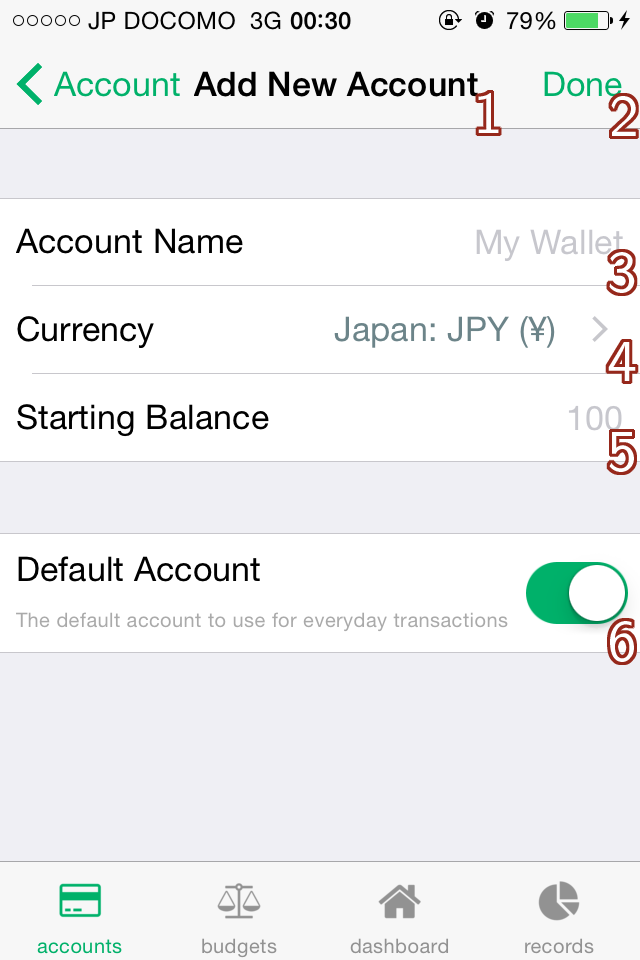
\includegraphics[scale=0.35]{ACC-0001-1} 
  \caption{Add New Account Screen}
  \label{fig:sub-account-1}
\end{subfigure}
\begin{subfigure}{0.5\textwidth}
  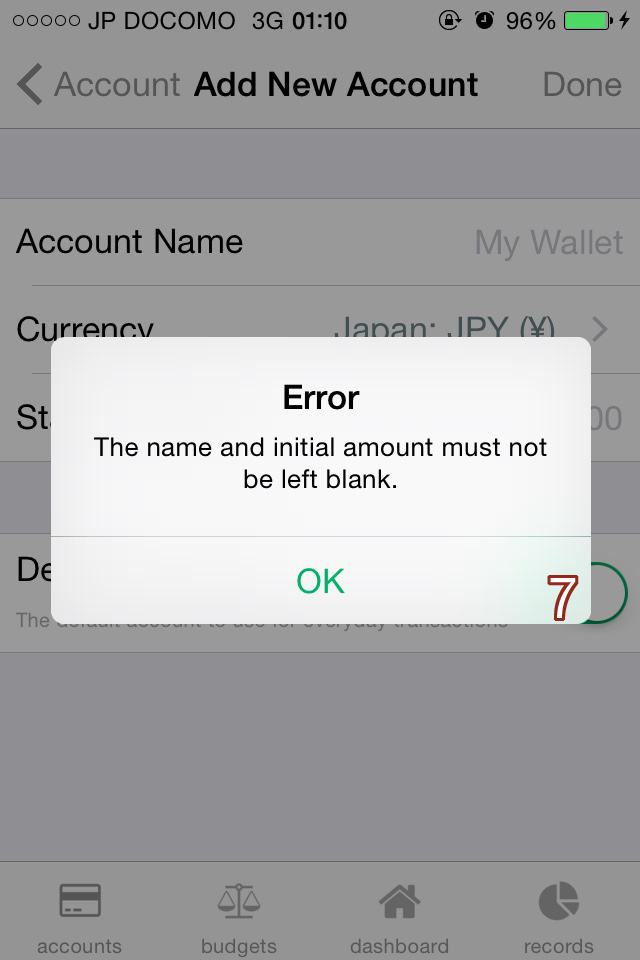
\includegraphics[scale=0.35]{ACC-0001-4}
  \caption{Error Scenario}
  \label{fig:sub-account-2}
\end{subfigure}
\caption{Add New Account Screenshots}
\end{figure}

\screentable{
	\header{Screen Component}
    	{Type}
        {Description}
    \row{1. Screen Title}
    	{Label Title}
        {Localization Key: MENULABEL\_ADD\_ACCOUNT}
    \row{2. Done Button}
    	{Button}
        {When tapped, the app checks on whether or not both the Account Name and the Initial Amount have been filled. \doublenewline
        If both textfields have been filled, then all fields (that is: account name, currency, initial amount, is default) will be saved into the core data. If not, then an error will pop up, prompting the user to have both textfields filled up. \doublenewline
        Localization Key: BUTTON\_DONE
        } 
    \row{3. Account Name Cell}
    	{Table Cell}
        {This table cell consists of two UI elements: A label and a textfield. \doublenewline
        
        Tap anywhere in the cell and the textfield will be placed in focus, bringing up a QWERTY keyboard. Tap anywhere outside the cell to dismiss the keyboard. \doublenewline
        
        The textfield has a character limit of 25 characters.\doublenewline
        
        Localization Keys: LABEL\_NAME, TEXTFIELD\_NAME\_PLACEHOLDER} 
    \row{4. Currency Cell}
    	{Table Cell}
        {This table cell consists of two label UI elements. \doublenewline
        
        When this table cell is tapped, the cell will be briefly filled with a light green background, then fade out as the screen transitions to the Currency Selection screen. The default currency depends on the user's device locale.\doublenewline 
        
        Localization Key: LABEL\_CURRENCY} 
}

\screentable{
	\header{Screen Component}
    	{Type}
        {Description}
    \row{5. Initial Amount Cell}
    	{Table Cell}
        {This table cell consists of two UI elements: A label and a textfield. \doublenewline
        
        Tap anywhere in the cell and the textfield will be placed in focus, bringing up a keyboard that is numeric with a decimal point.  Tap anywhere outside the cell to dismiss the keyboard. \doublenewline
        
        The textfield has a character limit of 15 characters.\doublenewline
         
        Localization Keys: LABEL\_STARTING\_BALANCE, TEXTFIELD\_STARTING\_BALANCE\_ PLACEHOLDER} 
    \row{6. Default Account Cell}
    	{Table Cell}
        {This table cell consists of three UI elements: two labels and a switch. The switch is turned off by default.\doublenewline
        
        Tap anywhere in the cell and the switch will be toggled. There can only be one default account at any time. \doublenewline
        
        Localization Keys: LABEL\_IS\_DEFAULT\_ACCOUNT, LABEL\_IS\_DEFAULT\_ACCOUNT\_ DESCRIPTION} 
    \row{7. Error Alert}
    	{Alert Controller}
        {This alert controller has two labels. \doublenewline
        
        The alert is displayed when either the account name or the initial amount has not been filled, and the user taps "Done".\doublenewline
        
        Localization Keys: ERRORLABEL\_ERROR\_TITLE, ERRORLABEL\_NAME\_CURRENCY\_ NOT\_EMPTY}
}

\subsubsection{Error Scenarios}

\errortable{
	\errorheader{Title}{Description}
    \errorrow{Duplicate Account Name}
    	{This error is triggered when the Done button is pressed and a similar account name already exists in the Core Data. \doublenewline
        
        Localization Key: ERRORLABEL\_ DUPLICATE\_ACCOUNT\_NAME}
    \errorrow{Duplicate Account Name}
    	{This error is triggered when the Done button is pressed and the account name or the amount has not been filled. \doublenewline
        
        Localization Key: ERRORLABEL\_NAME\_CURRENCY\_ NOT\_EMPTY}
    
    \errorrow{Multiple Decimals}
    	{No error alert is displayed, but this check exists in the textfield, where decimals can only be input once.}
        
    \errorrow{Maximum Length}
    	{No error alert is displayed, but this check exists in the textfield, where there is a maximum length for the textfield.}
}

\subsubsection{Use Cases}
